%; whizzy chapter
% -initex iniptex -latex platex -format platex -bibtex jbibtex -fmt fmt
% $B0J>e(B whizzytex $B$r;HMQ$9$k>l9g$N@_Dj!#(B

%     Tokyo Debian Meeting resources
%     Copyright (C) 2011 Junichi Uekawa
%     Copyright (C) 2011 Nobuhiro Iwamatsu

%     This program is free software; you can redistribute it and/or modify
%     it under the terms of the GNU General Public License as published by
%     the Free Software Foundation; either version 2 of the License, or
%     (at your option) any later version.

%     This program is distributed in the hope that it will be useful,
%     but WITHOUT ANY WARRANTY; without even the implied warranty of
%     MERCHANTABILITY or FITNESS FOR A PARTICULAR PURPOSE.  See the
%     GNU General Public License for more details.

%     You should have received a copy of the GNU General Public License
%     along with this program; if not, write to the Free Software
%     Foundation, Inc., 51 Franklin St, Fifth Floor, Boston, MA  02110-1301 USA

%  preview (shell-command (concat "evince " (replace-regexp-in-string "tex$" "pdf"(buffer-file-name)) "&"))
% $B2hA|%U%!%$%k$r=hM}$9$k$?$a$K$O(Bebb$B$rMxMQ$7$F(Bboundingbox$B$r:n@.!#(B
%(shell-command "cd image201205; ebb *.png")

%%$B$3$3$+$i%X%C%@3+;O!#(B

\documentclass[mingoth,a4paper]{jsarticle}
\usepackage{monthlyreport}

% $BF|IU$rDj5A$9$k!"Kh7nJQ$o$j$^$9!#(B
\newcommand{\debmtgyear}{2012}
\newcommand{\debmtgmonth}{5}
\newcommand{\debmtgdate}{19}
% (+ (* (- 2012 2005) 12) 5 -1) started from zero
\newcommand{\debmtgnumber}{88}

\begin{document}

\begin{titlepage}
\thispagestyle{empty}
% $B%?%$%H%k%Z!<%8(B:$BJT=8I,MW$JItJ,$O:G=i$N%^%/%m$KHt$P$9$3$H(B

\vspace*{-2cm}
$BBh(B\debmtgnumber{}$B2s(B $BEl5~%(%j%"(B Debian $BJY6/2q;qNA(B\\
\hspace*{-2cm}
\includegraphics[width=210mm]{image201003/debsen.eps}\\
\hfill{}\debmtgyear{}$BG/(B\debmtgmonth{}$B7n(B\debmtgdate{}$BF|(B

% $B$3$3$O%"%C%W%G!<%H$9$k$3$H(B
% $BA43QJ8;z$K$7$J$$$H%U%)%s%H$N%5%$%:$,9g$o$J$$$N$GCm0U(B
% TODO(uekawa): $B$J$s$G$=$&$J$k$N$+3NG'(B
\rotatebox{10}{\fontsize{32}{32} {\gt $BFC=8#1(B: XXXX}}

\rotatebox{10}{\fontsize{32}{32} {\gt $BFC=8#2(B: YYYY}}

\vspace*{-2cm}
\hfill{}
\includegraphics[height=6cm]{image200502/openlogo-nd.eps}
\end{titlepage}

% Title should be in Japanese text so that we can use it as lint for PDF shiori.
\dancersection{$B$O$8$a$K(B}{$B>e@n(B $B=c0l(B}

\begin{multicols}{2}
 

 $B:#7n$N(BDebian$BJY6/2q$X$h$&$3$=!#$3$l$+$i(BDebian$B$N@$3&$K$"$7$rF'$_F~$l$k$H(B
 $B$$$&J}$b!"$9$G$K$I$C$W$j$H$D$+$C$F$$$k$H$$$&J}$b!"7n$K0l2s(BDebian$B$K$D$$(B
 $B$F8l$j$^$;$s$+!)(B

 Debian$BJY6/2q$NL\E*$O2<5-$G$9!#(B

 \begin{itemize}
 \item \underline{Debian Developer} ($B3+H/<T(B)$B$N0i@.!#(B
 \item $BF|K\8l$G$N!V(B\underline{$B3+H/$K4X$9$k>pJs(B}$B!W$r@0M}$7$F$^$H$a!"%"%C%W%G!<%H$9$k!#(B
 \item \underline{$B>l(B}$B$NDs6!!#(B
 \begin{itemize}
  \item $BIaCJ$P$i$P$i$J>l=j$K$$$k?M!9$,(B face-to-face $B$G=P2q$($k>l$rDs6!(B
	$B$9$k!#(B
  \item Debian $B$N$?$a$K$J$k$3$H$r8l$k>l$rDs6!$9$k!#(B
  \item Debian$B$K$D$$$F8l$k>l$rDs6!$9$k!#(B
 \end{itemize}
 \end{itemize}		

 Debian$B$NJY6/2q$H$$$&$3$H$G5f6KE*$K$O;22C<TA40w$,(BDebian Package$B$r$,$j$,$j(B
 $B$H:n$k%9!<%Q!<%O%C%+!<$K$J$C$?;Q$rLQA[$7$F$$$^$9!#>pJs$N6&M-!&3hMQ$rDL$7(B
 $B$F(B Debian$B$N:#8e$NG=F0E*$JE83+$X$NEZBf$H$7$F!"!V>l!W$H$7$F$N6u4V$rDs6!$9(B
 $B$k$N$,L\E*$G$9!#(B

\end{multicols}

\newpage

\begin{minipage}[b]{0.2\hsize}
 \definecolor{titleback}{gray}{0.9}
 \colorbox{titleback}{\rotatebox{90}{\fontsize{80}{80} {\gt $B%G%S%"%sJY6/2q(B} }}
\end{minipage}
\begin{minipage}[b]{0.8\hsize}
\hrule
\vspace{2mm}
\hrule
\begin{multicols}{2}
\tableofcontents
\end{multicols}
\vspace{2mm}
\hrule
\end{minipage}

\dancersection{$B;vA02]Bj(B}{$B4d>>(B $B?.MN(B}

$B:#2s$N;vA02]Bj$O0J2<$G$9(B:
\begin{enumerate}
 \item hogefuga
\end{enumerate}
$B$3$N2]Bj$KBP$7$FDs=P$$$?$@$$$?FbMF$O0J2<$G$9!#(B
\begin{multicols}{2}
{\small
 %; whizzy-master ../debianmeetingresume201205.tex
% $B0J>e$N@_Dj$r$7$F$$$k$?$a!"$3$N%U%!%$%k$G(B M-x whizzytex $B$9$k$H!"(Bwhizzytex$B$,MxMQ$G$-$^$9!#(B
%

\begin{prework}{ BeatenAvenue }

1.$B$*$9$9$aK\!'(B

$B!V(Bwindows$B%W%m%U%'%C%7%g%J%k%2!<%`%W%m%0%i%_%s%0(B($BA4#24,(B?)$B!W(B
DirectX$B4XO"$NFbMF$b$"$C$?5$$,$7$^$9$,(Bwin32API$B$K$D$$$F$NFbMF$,B?$+$C$?5$$,$7$^$9!#@N$NK\$G$9$,%?%9%/=hM}$N9M$(J}$J$I8=:_$G$bDLMQ$9$kItJ,$OB?$$$H;W$$$^$9!#$3$NK\$rGc$C$F$+$i(BC++$B$NJY6/$r;O$a$?$3$H$b$"$C$F!&!&!&8D?ME*$K;W$$=P$,$?$/$5$s$"$j$^$9!#(B

$B!V(BDirectX$B5U0z$-BgA4(B500$B$N6K0U!W(B
$BF~LgE*$JM%$7$$2r@b$+$i0lJbF'$_9~$s$@%W%i%9%"%k%U%!$^$GB7$C$F$$$^$9!#;DG0$J$,$i@dHG$G?^=q4[$+$i<Z$j$FFI$_$^$7$?!#(BDirectX9$B$N2r@b=q$G$O0lHV$h$$$b$N$+$H;W$$$^$9!#(B

$B!V(BGameProgrammingGems($B%7%j!<%:(B)$B!W(B
$B3$30$N%2!<%`%W%m%0%i%^$NJ}!9$,=q$$$?5-;v$r$^$H$a$?K\!#(B3$B4,$@$C$?$+$H;W$$(B
 $B$^$9$,(BNaughty Dog$B$NJ}$,=q$$$?(B"Jak and Daxter: The Precursor legacy"$B$G$N%^%C%W0\F0=hM}$K$D$$$F$NFbMF$,9%$-$G$9!#$*CMCJ0J>e!#(B

2.$B=i?4<T$K$*$9$9$a$9$k%9%/%j%W%H8@8l!'(B
Debian$B$H$OA4$/4X78$J$$$G$9$,(BDOS$B%P%C%A%U%!%$%k$H(BExcelVBA$B$N$A$g$C$H$7$?;H$$J}$O3P$($J$$$H;vL3;E;v$,?J$_$^$;$s!#2r@b%5%$%H$bB?$$$N$GIU$-$C$-$j$G65$($kI,MW$b$"$^$j$J$$$G$9!#(B
Linux$B$@$H(Bbash$B$N%9%/%j%W%H$J$s$G$7$g$&$+!#;d$,=i?4<T$J$N$G$=$l$7$+?($C$F$$$^$;$s!&!&!&!#(B
\end{prework}

\begin{prework}{ amotoki }

1. $B:rF|M'?M$+$i4+$a$i$l$F5$$K$J$C$F$$$k$N$,!V>pG.%W%i%0%i%^!<!W$G$9!#<+J,$N?M@8$r<+J,$G@Z$j3+$$$F$$$/$?$a$KI,MW$J$3$H$,J,$+$j$d$9$/@0M}$5$l$F$$$k$1$I!"<+J,$rA0$K?J$a$F$/$l$k>pG.$r46$8$?$H$N$3$H!#$5$C$=$/CmJ8$7$?!#(B

2. $B:#$*$9$9$a$9$k$H$7$?$i(BPython$B$r$*A&$a$7$^$9!#%*%V%8%'%/%H;X8~$b=q$-$d$9$$$7!"%i%$%V%i%j$b=<<B$7$F$$$F!"%^%K%e%"%k$b<BNc$,$=$m$C$F$$$k$N$G!"%W%m%0%i%_%s%0$r3X$s$G$$$/>e$G$h$$$H;W$$$^$9!#Bg$-$a$N(BOSS$B%W%m%8%'%/%H$G$b;H$o$l$F$$$k$N$G!"CN$C$F$*$$$FB;$9$k$3$H$b$"$j$^$;$s!#:G=i$N0lJb$H$7$F$O!V(BPython$B%A%e!<%H%j%"%k!W$,$h$$$H;W$$$^$9!#:#$G$b$H$-$I$-8+$k$3$H$,$"$j$^$9!#(B
\end{prework}

\begin{prework}{ $B5HLn(B(yy\_y\_ja\_jp) }

1. Git$B$K$h$k%P!<%8%g%s4IM}(B $B<B:]$N%W%m%8%'%/%H$G$N(BGit$B$NMxMQK!$,=q$+$l$F$$$k$h$&$G$9!%(B

2. $B%7%'%k%9%/%j%W%H(B
$B5$7Z$K;H$($k$+$i$G$9!%(B
bash(1), dash(1)
\end{prework}

\begin{prework}{ dictoss($B?yK\!!E5=<(B) }

1.$B!V%$%s%F%k(B $B%9%l%C%G%#%s%0!&%S%k%G%#%s%0!&%V%m%C%/(B -- $B%^%k%A%3%";~Be$N(BC++$BJBNs%W%m%0%i%_%s%0!W%*%i%$%j!<!&%8%c%Q%s!"(BJames Reinders$BCx(B
Intel$B$,3+H/$78=:_$O(BGPLv2$B$G8x3+$7$F$$$k(BC++$B$NJBNs7W;;MQ%i%$%V%i%j!V(BThreading Building Blocks$B!W$N2r@b$r9T$C$F$$$kK\!#%^%k%A%3%";~Be$NCf$GJ#?t$N(BCPU$B%3%"$r8zN(E*$K;HMQ$7$F7W;;@-G=$r>e$2$k$?$a$NCN<1$,5M$^$C$F$$$k!#$"$/$^$GC10l%N!<%I$G7W;;@-G=$r>e$2$k$?$a$N<jK!$G$"$j!"J#?t%N!<%I$G7W;;@-G=$r8~>e$5$;$k%/%i%9%?%j%s%05;=Q$NOC$G$O$J$$$N$GCm0U!#(B

2.$B$*4+$a$O(Bpython$B!#M}M3$O%W%m%0%i%_%s%0=i?4<T$H$$$&$3$H$G3+H/<T$K$h$C$F=q$-J}$K:90[$,=P$K$/$$J,(Bweb$B$G>R2p$5$l$F$$$k%3!<%I$KJJ$,$J$/$H$C$D$-$d$9$$$?$a!#(B
$B$*$9$9$a%5%$%H$O!"$&!<$s!"$J$s$G$7$g!)<+J,$OJL$N8@8l$,=q$1$k$h$&$K$J$C$F$+$i(Bpython$B$r;O$a$?$N$G(B"\url{http://www.python.jp/doc/release/}"$B$r3NG'$7$^$9!#(B
\end{prework}

\begin{prework}{ kamonshohei }

1. $B%7%'%k%9%/%j%W%H%7%'%k%9%/%j%W%H4pK\%j%U%!%l%s%9(B

2. $B%7%'%k%9%/%j%W%H$G$7$g$&$+!#%j%J%C%/%9$N%3%^%s%I$@$1$G!"$A$c$A$c$C$H<BAu$G$-$k<j7Z$5$,$$$$$G$9!#:G=i$N0lJb$G0FFb$9$k=q@R$O(B 1$B$G$"$2$?%7%'%k%9%/%j%W%H4pK\%l%U%!%l%s%9$G$9!#(B
\end{prework}

\begin{prework}{ emasaka }

1. $B%1%s!&%9%_%9!VC/$b65$($F$/$l$J$$@;=q$NFI$_J}!W!#@;=q$K=q$+$l$F$$$k$=$N$^$^$NJ8LL$r??LLL\$KFI$s$G%f!<%b%i%9$K>R2p!J!)!K$7$F$$$kK\!J(BDebian$B4X78$J$$!K(B

2. Bash$B$H=q$3$&$+$H;W$C$?$1$I(BRuby$B!#M}M3$O!V%*%V%8%'%/%H;X8~$r;H$C$F$b;H$o$J$/$F$b$$$$!W$G$O$J$/$F!V%*%V%8%'%/%H;X8~$r6/@)$5$l$k!W$+$i!#=q@R$O!V$?$N$7$$(BRuby$B!W(B

\end{prework}

\begin{prework}{ $BK\>1(B }

1. Debian $BJY6/2q;22C<T$K>R2p$7$?$$=q@R$r#1:}0J>e5s$2$F!"FbMF$r4JC1$K>R2p$7$F$/$@$5$$!#(B
$BDjHV$G$9$,!X%O%C%+!<$H2h2H!Y$H$+$I$&$G$7$g$&!#%*%?%/$N1eG0$,9~$a$i$l$F$$$^$9!#?F$H$7$F;R6!$N>-Mh$KIT0B$r46$8$^$9!#(B

2. $B$"$J$?$,2?$+%9%/%j%W%H8@8l$r%W%m%0%i%_%s%0=i?4<T$K$*4+$a$9$k$H$7$F!V$=$N8@8l$rA*$s$@M}M3!W$H!V:G=i$N0lJb$H$7$F0FFb$9$k=q@R!?%5%$%H!W$r65$($F$/$@$5$$!#(B
PHP$B$,$*$9$9$a$G$9!#$[$+$KHf$Y$F;E;v$,B?$=$&$H$$$&M}M3$G$9!#B?$$$+$I$&$+$O<B:]$N$H$3$m$o$+$j$^$;$s$,!"(B

\url{http://www.google.co.jp/trends/?q=PHP,+Perl,+Python,+Ruby,+Javascript,+Haskell&ctab=0&geo=jp&geor=all&date=ytd&sort=0}

$B$3$38+$k$HB?$=$&$G$9!#0FFb$9$k=q@R$H$7$FDjHV$O%^%s%b%9K\$@$H;W$$$^$9$,!"FI$s$@$3$H$O$"$j$^$;$s!#$=$7$F8E$$>pJs$+$b$7$l$^$;$s!#(B
$B0JA0!"$H$"$k(BPHP$BJ}LL$NJ}$H$*OC$7$9$k5!2q$,$"$j!"%*%i%$%j!<$NK\$O$A$g$C$H!DE*$J$3$H$rOC$7$?$i!"!V$"$"$$$&K\$b$$$$$+$J$H;W$C$F$^$9!W$H$$$o$l$^$7$?!#K]Lu<T$G$7$?!#(B

\end{prework}

\begin{prework}{ henrich }

1. $B!VF~Lg(BDebian$B%Q%C%1!<%8!W!#=qL>$+$iFbMF$,J,$+$k$+$H$O;W$$$^$9$,!"(BDebian$B%Q%C%1!<%8$N:n$jJ}$N=q@R$G$9!#B34)$,4|BT$5$l$^$9(B

2. Python $B$rA*$S$^$7$?!#(BPerl$B$O?M$K$h$C$F$H$F$b=q$-J}$,JQ$o$k$H$3$m$,$"$^$j4r$7$/$J$/!"(BRuby$B$O%P!<%8%g%s4V$N0\9T$,<c43MpK=$K46$8$i$l$?$N$G!#2?EY$b%W%m%0%i%_%s%0$K:C@^$7$F$$$k;d$G$9$,!":#2s(BPython$B$r3X$V$N$KA*$s$@!V=i$a$F$N%3%s%T%e!<%?%5%$%(%s%9!W$,$H$F$bNI$$=q@R$G$7$?!#(B
\end{prework}

\begin{prework}{ $BLnEg!!5.1Q(B }

1.$B!V%$%N%Y!<%7%g%s$N%8%l%s%^!W!J(BISBN10:4798100234)$B$H!"!V$N$&$@$^!W(B(ISBN10:4344015959)$B!#!V%$%N%Y!<%7%g%s$N%8%l%s%^!W$O!"5;=Q3W?7$,4{B8$N$b$N$r$V$A2u$7$F$$$/2aDx$K$*$$$F!"4{B85;=Q$K$*$$$FM%=($JAH?%$G$"$l$P$"$k$[$I5;=Q3W?7$K$D$$$F$$$1$J$/$J$C$F$7$^$&8=>]$rM}5M$a$G@bL@$7$?K\!#!V$N$&$@$^!W$O?M$N9TF0$K$*$$$F$O!"<B$O=,47$,@h$G$d$k5$$O8e$+$i$D$$$F$/$k$b$N$G$"$k$H$$$&;v$r@bL@$7$?K\!#(B

2. $B%W%m%0%i%_%s%0=i?4<T$K$O:#;~$N>u67$+$i(Bjavascript/HTML5$B$r4+$a$?$$$N$G$9$,!"4N?4$N<+J,$,L$I>2A!#:G=i$N0lJb$O%2!<%`M7$S$?$5$K%W%m%0%i%`3P$($?7P83$r85$K!"(B\url{http://wise9.jp/}$B!!$H!"!!(B\url{http://enchantjs.com/}$B!!$,$*$9$9$a$J$N$+$J!)(B
\end{prework}

\begin{prework}{ yamamoto }

1. Debian $BJY6/2q;22C<T$K>R2p$7$?$$=q@R$r#1:}0J>e5s$2$F!"FbMF$r4JC1$K>R2p$7$F$/$@$5$$!JFC$K5;=Q=q$K$O8B$j$^$;$s!K!#(B

$BM-L>$@$H;W$&$N$G!">R2p$9$k$[$I$N$3$H$O$J$$$+$b$7$l$^$;$s$,!"!VF~Lg(BUNIX$B%7%'%k%W%m%0%i%_%s%0(B-$B%7%'%k$N4pAC$+$i3X$V(BUNIX$B$N@$3&!!(BBruce Blinn $BCx!&;32<E/E5(B $BLu!W$r0&FI$7$F$$$^$9!#$^$"!"%7%'%k%9%/%j%W%H%W%m%0%i%_%s%0$r%7%'%k%W%m%0%i%_%s%0$H8@$C$F$$$k%?%$%H%k(B ($BL^O@%7%'%k<+BN$N2r@b$b$"$j$^$9$1$I$M(B) $B$O%"%l$G$9$,!"(BB$B%7%'%k$N%9%/%j%W%H$r=q$/$H$-$K$ONI$/3+$$$F$$$^$9!#(B

2. $B$"$J$?$,2?$+%9%/%j%W%H8@8l$r%W%m%0%i%_%s%0=i?4<T$K$*4+$a$9$k$H$7$F!V$=$N8@8l$rA*$s$@M}M3!W$H!V:G=i$N0lJb$H$7$F0FFb$9$k=q@R!?%5%$%H!W$r65$($F$/$@$5$$!#(B

\#!/bin/sh $BK|:P!*(B
$B$I$3$G$bBg35F0$/$+$i$*$9$9$a!#(B
B$B%7%'%k$N:nK!$K=>$C$F$$$l$P!":#$N(Bdash$B$J$iBgBNF0$/!)$_$?$$(B ($BL$3NG'(B)$B!#(B
$B$@$a$J$i!!(B\#!/bin/bash$B$G!#(B
$B$H$+$$$$$J$,$i$b!"$*$$$i$N%7%'%k%9%/%j%W%H$K$O30It%3%^%s%I%P%j%P%jF~$l$F$^$9$1$I!#(B($B$&$R(B

$B>e5-$N=q@R$G$b$$$$$G$9$,!"$0$0$k$5$s$K$*;G$$$7$?$i!";29M$K$J$k%5%$%H$O;3$[$I=P$F$/$k$G$7$g$&!#(B
\end{prework}

}
\end{multicols}

\dancersection{$B:G6a$N(BDebian$B4XO"$N%_!<%F%#%s%0Js9p(B}{$B4d>>(B $B?.MN(B}
\subsection{$BEl5~%(%j%"(BDebian$BJY6/2q(B86$B2sL\Js9p(B}

% (query-replace-regexp "<.*?>" "")
% (query-replace-regexp "^[	 ]\+" "")


\dancersection{Debian Trivia Quiz}{$B4d>>(B $B?.MN(B}

$B$H$3$m$G!"$_$J$5$s(B Debian $B4XO"$NOCBj$K$*$$$D$$$F$$$^$9$+!)(BDebian$B4XO"$NOC(B
$BBj$O%a!<%j%s%0%j%9%H$r$h$s$G$$$k$HDI@W$G$-$^$9!#$?$@$h$s$G$$$k$@$1$G$O$O(B
$B$j$"$$$,$J$$$N$G!"M}2rEY$N%F%9%H$r$7$^$9!#FC$K0l?M$@$1$G$O0UL#$,$o$+$i$J(B
$B$$$H$3$m$b$"$k$+$bCN$l$^$;$s!#$_$s$J$G0l=o$KFI$s$G$_$^$7$g$&!#(B

$B:#2s$N=PBjHO0O$O(B\url{debian-devel-announce@lists.deban.org} $B$d(B \url{debian-devel@lists.deban.org}$B$KEj9F$5$l$?(B
$BFbMF$H(BDebian Project News$B$+$i$G$9!#(B

\begin{multicols}{2}
% %; whizzy-master ../debianmeetingresume201211.tex
% $B0J>e$N@_Dj$r$7$F$$$k$?$a!"$3$N%U%!%$%k$G(B M-x whizzytex $B$9$k$H!"(Bwhizzytex$B$,MxMQ$G$-$^$9!#(B
%

\santaku
{DebConf13 $B$N3+:ECO$H3+:EF|$O!)(B}
{$BF|K\!"El5~ET(B 6$B7n(B20$BF|(B}
{$B%K%+%i%0%"(B $B%^%J%0%"(B 7$B7n(B8-14$BF|(B}
{$B%9%$%9!"%t%)!<%^%k%-%e(B 8$B7n(B11-18$BF|(B}
{3}
{$B%K%+%i%0%"$O(BDebConf12$B$N3+:ECO$G$9!#(B
DebConf13$B$O%9%$%9$N%-%c%s%WCO$G3+:E$G$9!#(B
6/20$B$O3'$5$sM=Dj$r6u$1$F$*$-$^$7$g$&!#(B}

\santaku
{$B@$3&$N(BWeb$B%5!<%P$G:G$b?M5$$N$"$k(BLinux $B%G%#%9%H%j%S%e!<%7%g%s(B(W3Techs$BD4$Y(B)$B$O!)(B}
{CentOS}
{Debian}
{Ubuntu}
{B}
{\url{http://w3techs.com/technologies/history_details/os-linux}$B$K7k2L$N%0%i%U$,$"$j$^$9!#(B
$B8=:_(B Linux $B$r;HMQ$7$F$$$k(B web $B%5!<%P$N(B 32.9\% $B$,(B Debian $B$rMxMQ$7$F$*$j!"$=$N3d9g$O8=:_$bA}2C$rB3$1$F$$$k$=$&$G$9!#(B}

\santaku
{Debian $B%+!<%M%k%A!<%`$N%a%s%P!<$G$"$j!"(Bkernel.org $B$N(B 3.2.y $B0BDjHG7ONs$N%a%s%F%J$G$b$"$k(B Ben Hutchings $B$5$s$,<!4|(B Debian $B0BDjHG$H0l=o$K=P2Y$5$l$k(B Linux $B%+!<%M%k$K(B (3.2 $B7ONs$N(B mainline $B$K$OL5$$(B) $BDI2C5!G=$,Ek:\$5$l$kM=Dj$G$"$k$H=R$Y$F$$$^$9!#(B
$BB?$/$NDI2CE@$NCf$K4^$^$l$J$$$b$N$O2?!)(B}
{PREEMPT\_RT}
{Hyper-V guest drivers$B$N6/2=(B}
{ARM64/AArch64$B%"!<%-%F%/%A%c%5%]!<%H(B}
{C}
{Hyper-V guest drivers$B$O(Bmainline kernel$B$G(B3.2$B$K$b4^$^$l$F$$$^$9$,!"$h$j2~A1$5$l$?(B3.4$B$+$i$N=$@5$,F3F~$5$l$^$9!#(B
PREEMPT\_RT$B$O%O!<%I%j%"%k%?%$%`$r<B8=$9$k$?$a$N(BPatch$B!"(B
linux-image-rt-amd64 , linux-image-rt-686-pae $B$N(Bmetapackage$B$G;HMQ$G$-$^$9!#(B
$B?7$7$$(BARM 64$B%S%C%H%"!<%-%F%/%A%c%5%]!<%H$O(Bmainline kernel 3.7$B$+$i(B}

\santaku
{Wookey$B$5$s$,%"%J%&%s%9$7$?(Balpha$BHG$N(BDebian port arm64 image$B$O!)(B}
{Debian/Ubuntu port image}
{Debian/KFreeBSD port image}
{Debian/GnuHurd port image}
{A}
{self-bootstrapp(non x86)$BBP1~$H$N$3$H$G$9!#(B\url{http://wiki.debian.org/Arm64Port}$B$G%9%F!<%?%9$,3NG'$G$-$^$9!#(B}

\santaku
{700,000$BHVL\$N%P%0$,Js9p$5$l$?F|$rEv$F$k(B700000thBugContest$B$N7k2L$,=P$^$7$?!#$=$NM=A[F|$HJs9pF|$O!)(B}
{2012/12/12$B$rM=A[$7$?(BDavidPrevot}
{$BM=A[F|(B:2013/02/04$B!"Js9pF|(B:2013/02/14}
{$BM=A[F|(B:2013/02/07$B!"Js9pF|(B:2013/02/14}
{$BM=A[F|(B:2013/02/14$B!"Js9pF|(B:2013/02/07}
{C}
{$B:G$b6a$$(B2013/02/14$B$rM=A[$7$?(BChristian Perrier$B$5$s$,Ev$F$^$7$?!#7k2L$O(B\url{http://wiki.debian.org/700000thBugContest}$B$G8x3+$5$l$F$$$^$9!#(B
$B$^$?!"(B800,000/1,000,000$BHVL\$N%P%0$,Js9p$5$l$kF|$rEv$F$k%3%s%F%9%H(B\url{http://wiki.debian.org/800000thBugContest}$B$b3+:E$5$l$F$$$^$9!#(B}

\santaku
{master.debian.org$B$,?7$7$$5!3#$K0\9T$5$l$^$7$?!#$3$l$O2?$N%5!<%P$G$7$g$&$+(B $B!)(B}
{@debian.org$B$N%a!<%k%5!<%P(B}
{$B%Q%C%1!<%8$N%^%9%?!<%5!<%P(B}
{$B%Q%C%1!<%8$N%9%]%s%5!<(B(mentor)$B$rC5$9%5!<%P(B}
{A}
{$B8E$$%5!<%P$O%G%#%9%/>c32Ey$,$"$C$?$N$G!"<wL?$HH=CG$5$l!"%G!<%?$,B;<:$9$kA0$K?7$7$$%5!<%P$K0\9T$5$l$^$7$?!#(Bftp-master.debian.org$B$O(BDebian$B$N(B official package $B%j%]%8%H%j$G$9!#%Q%C%1!<%8$N%9%]%s%5!<(B(mentor)$B$rC5$9$N$O(Bmentors.debian.net$B!#(B }

\santaku
{pbuilder$B$K(Bclang support$B$,DI2C$5$l$^$7$?!#C/$,=q$$$?%Q%C%A$G$7$g$&$+!)(B}
{Sylvestre Ledru}
{Junichi Uekawa}
{Hideki Yamane}
{C}
{Debian$B$N(BClang$B%5%]!<%H$OCe!9$H?J$s$G$$$^$9!#(B}

\santaku
{DPN - 2013$BG/(B3$B7n(B4$BF|9f$K<h$j>e$2$i$l$?F|K\$N%$%Y%s%H$O(B}
{Open Source Conference 2013 Tokyo/Spring}
{Open Source Conference 2013 Hamamatu}
{Open Source Conference 2013 Tokushima}
{A}
{\url{http://henrich-on-debian.blogspot.jp/2013/02/open-source-conference-2013-tokyospring.html} $B>\:Y$O8e$[$I!#(B}


\end{multicols}

%-------------------------------------------------------------------------------
\dancersection{Python$B=i?4<T$,!V(BPython$B%W%m%U%'%C%7%g%J%k%W%m%0%i%_%s%0!W$rFI$s$G$_$?(B}{$B$d$^$M$R$G$-(B}
%-------------------------------------------------------------------------------
\label{sec:python-professional-programing}
\index{python}

$B$o$?$/$7!"!V(BPython$B%W%m%U%'%C%7%g%J%k%W%m%0%i%_%s%0!W$H$$$&=q@R$r@hF|9XF~$7$^$7$?!#;d<+?H$O$^$@(B3$B7nKv$0$i$$$K(BPython$B$NF~Lg$+$i;O$a$?$P$+$j$GK\Ev$O(BPython$B%S%.%J!<%:%W%m%0%i%_%s%0$,M_$7$$$N$G$9$,!"$^$@@$$NCf$K$O$=$N$h$&$JK\$O$"$j$^$;$s$7!"$3$N=q@R<+BN$OI>H=$,NI$+$C$?$N$G!D(B

$B$G!"<B:]FI$s$G$_$FCf!9<BA)E*$H$$$&$+4D6-9=C[$J$I$G;29M$K$J$k$3$H$,B?!9$"$j$^$7$?!#$7$+$7!"$b$&$A$g$C$HFM$C9~$s$G$_$?$$$J$!!"$H$$$&$H$3$m$,$$$/$D$+$"$C$?$N$G!"(BDebian$B%Q%C%1!<%8J}LL$+$i$N8+J}$H$7$F<h$j>e$2$F$_$h$&$H;W$$$^$9!#$3$N=q@R<+BN$G$O(BUbuntu11.10$B$r;H$C$F$$$^$9$,!";d$N(BDebian unstable$B$N$d$jJ}$G$bBgBN$N$H$3$m$O$=$N$^$^1~MQ$,8z$/$O$:$G$9!#(B


\subsection{$B$J$k$Y$/%G%#%9%H%j%S%e!<%7%g%s$N%Q%C%1!<%8$r;H$$$?$$(B}

Python$B$K$O(BPython$B%Q%C%1!<%8$,$"$j!"G[I[%5%$%H(BPyPI$B$,$"$j$^$9!#(BPerl$B$K(BCPAN$B!"(BRuby$B$K(Bgems$B!"(BR$B$K(BCRAN$B$_$?$$$J$b$N$G$9$M!#$G!"$3$N(BPython$B%Q%C%1!<%8$rF3F~$9$k$N$K(Bpip$B$H$$$&%D!<%k$r;H$&;]@bL@$,$"$k$N$G$9$,(B(P.4)$B!"(Bgithub$B$+$i(Bwget$B$7$F!"%$%s%9%H!<%k%9%/%j%W%H$r(Bsudo$B$G<B9T$7$F$$$^$9!#(B\verb!/usr/local! $B0J2<$K%D!<%k$,F~$k$o$1$G$9!#=q@RA4BN$G$3$N(Bpip$B$r;H$C$?%$%s%9%H!<%k$r4+$a$F$$$^$9$,!"$3$l$OH~$7$/$J$$!#(BDebian$B%Q%C%1!<%8$K(Bpython-pip$B$,$"$k$N$G!"$=$A$i$rF~$l$F$b$$$$$s$8$c$J$$$+$H;W$$$^$9(B\footnote{pip$B$O<c43%P!<%8%g%s$,8E$$$G$9$,!"$=$s$J$KITET9g$b$J$$$+$J!<$H!#8E$$$N$,7y$J$i%m!<%+%k$K%"%C%W%G!<%H%Q%C%1!<%8:n$C$A$c$&$N$,5H!#(B}$B!#$=$l$+$i%f!<%6!<$N(B HOME $B0J2<$K%Q%C%1!<%8$r%$%s%9%H!<%k$9$k(Bvirtualenv$B$H$$$&%D!<%k$,$"$j$^$9!#$3$l$b(Bpython-virtualenv$B%Q%C%1!<%8$rF~$l$FBP1~$7$^$9!#$3$N8e$O!"(Bvirtualenv$B$G%f!<%6!<$N(BPython$B4D6-$K(Bpip$B$G%Q%C%1!<%8$rF~$l$F$$$C$F$b$$$$$+$J!"$H;W$$$^$9!#JXMx%D!<%k$H$7$F>R2p$5$l$F$$$k(Bvirtualenvwrapper$B$b(Bvirtualenvwrapper$B%Q%C%1!<%8$,$"$j$^$9$N$G$=$l$rF~$l$A$c$$$^$7$g$&!#(B

\begin{commandline}
$ sudo apt-get install python-pip python-virtualenv virtualenvwrapper
\end{commandline}

$B$3$N8e$G%f!<%6!<8D?M$N(BPython$B2>A[4D6-2<$K(Bpip$B$G(BPython$B%Q%C%1!<%8$r%,%7%,%7F~$l$F$$$/$N$O$"$j$@$H;W$$$^$9!#(B


\subsection{$BJ#?t%P!<%8%g%s$N(BPython$B$r;H$&!"$N$O$$$$$1$I!#(B}

Python2.5$B$r%$%s%9%H!<%k$9$k$N$K8x<0$N%Q%C%1!<%8%j%]%8%H%j$+$i$@$H(B11.10$B$KF~$l$i$l$J$$$h!"$H$$$&$3$H$,=q$$$F$"$j$^$9(B(P.11)$B!#$3$3$G(BPPA$B$+$i%$%s%9%H!<%k$9$k$+!"%=!<%9$+$i%$%s%9%H!<%k$9$k$+$H$$$&A*Br$K$J$C$F$$$^$9!#6HL3$G;H$&>l9g!"$=$N(BPPA$B$,$I$l$[$I?.MQ$G$-$k$+$r@bL@$9$k$N$,Fq$7$$$h$&$K;W$$$^$9!#<+8J@UG$$G!"$C$F=q$$$F$"$j$^$9$,!"BgDqLUL\E*$K$=$N(BPPA$B?.MQ$7$A$c$&$h$&$J!D!#8E$$%P!<%8%g%s$r;H$o$J$-$c%@%a!"$H$$$&>l9g!";d$@$C$?$i!V(Bdebootstrap$B$G8E$$4D6-$r:n$k!W$H$$$&$d$jJ}$G$d$j$^$9!J(Bdebootstrap$B$K$D$$$F$O8e$[$I=R$Y$^$9!K!#(B


$B$=$l$+$i%=!<%9$+$i(BPython2.5$B$rF~$l$k@bL@$G$9$,!"(B

\begin{commandline}
$ wget http://www.python.org/ftp/python/2.5.6/Python-2.5.6.tgz
$ tar -xvzf Python-2.5.6.tgz
$ cd Python-2.5.6
$ LDFLAGS="-L/usr/lib/x86_64-linux-gnu" ./configure
$ make
$ sudo make install
($B!V(BPython$B%W%m%U%'%C%7%g%J%k%W%m%0%i%_%s%0!W$h$j0zMQ!K(B
\end{commandline}

$B$H$$$&@bL@$K$J$C$F$$$^$9!#(Bi386$B$@$H%Q%9JQ$o$k$h$M!D$H$$$&$N$OFI$_<h$l$k$N$+<c43?4G[$J=j$G$9!#%W%m%U%'%C%7%g%J%k$@$+$i$$$$$N$+$J!)I,MW$J0MB8%Q%C%1!<%8$K$D$$$F$O!":G=i$NJ}$N%Z!<%8$G(B

\begin{commandline}
$ sudo aptitude -y install build-essential
$ sudo aptitude -y install libsqlite3-dev
$ sudo aptitude -y install libreadline6-dev
$ sudo aptitude -y install libgdbm-dev
$ sudo aptitude -y install zlib1g-dev
$ sudo aptitude -y install libbz2-dev
$ sudo aptitude -y install sqlite3
$ sudo aptitude -y install tk-dev
$ sudo aptitude -y install zip
($B!V(BPython$B%W%m%U%'%C%7%g%J%k%W%m%0%i%_%s%0!W$h$j0zMQ!K(B
\end{commandline}
%$ -- for emacs

$B$H$J$C$F$$$^$7$?!#$"$!!"$3$l$O%$%1$F$J$$!#%Q%C%1!<%8%S%k%IMQ$N%Q%C%1!<%8<hF@$O(B build-dep $B$9$k$Y$-$G$9!#(BSqueeze$B$G$O$^$@(B2.5$B$N%P%$%J%j%Q%C%1!<%8$,<j$KF~$k$N$G!"$3$3$G$O(B2.4$B$r%?!<%2%C%H$K:n6H$7$F$_$^$7$g$&!#$3$s$JIw$K(B\footnote{$B$3$3$N%Q%C%1!<%8L>;XDj$O!"K\Ev$O(Bpython2.4$B$K$7$?$$$1$IL5$$$N$G(B2.5$B$K$7$F$$$^$9!#B?>/$N:9$O8e$G=$@5!#(B}$B!#(B

\begin{commandline}
$ sudo apt-get build-dep python2.5
\end{commandline}

$B$3$l$G(BPython$B$r%S%k%I$9$k$H$-$KI,MW$J0MB8%Q%C%1!<%8$O$9$Y$F%$%s%9%H!<%k$5$l$^$9!#$"!"(Bapt line$B$K(Bdeb-src$B%i%$%s$rDI2C$rK:$l$:$K!#$3$N$d$jJ}$J$i!"(BPython$B0J30$N%=%U%H%&%'%"%Q%C%1!<%8$G$b%P!<%8%g%s$,JQ$o$C$F$bBgBN1~MQ$,8z$-$^$9!#(B

$B$=$7$F!V%=!<%9$+$i$=$N$^$^F~$l$k$H(B\verb!/usr/local!$B0J2<$KF~$k$+$i!"(Bpython$B$H$@$1BG$D$H(BPATH$B$NM%@hEY$G%=!<%9$+$iF~$l$?(BPython2.5$B$,5/F0$9$k!W!D$H$$$&@bL@$,!D$=$s$Jf+:n$i$J$$J}$,$$$$$8$c$J$$$G$9$+!<!#;d$J$i%=!<%9$+$iF~$l$k$N$J$i!V(BPython2.5$B$N(BDebian$B%Q%C%1!<%8$rMxMQ4D6-MQ$K%j%S%k%I$7$F$$$l$k!W$r$d$j$^$9!#(BPTS$B$N(BPython2.4$B$N%Z!<%8(B \footnote{\url{http://packages.qa.debian.org/p/python2.4.html}} $B$+$i%=!<%9%Q%C%1!<%8$N(Bdsc$B%U%!%$%k$,<hF@$G$-$k$N$G!"$3$l$r(Bdevscripts$B%Q%C%1!<%8$N(Bdget$B%3%^%s%I$G<hF@$7$^$9!#(B

\begin{commandline}
$ sudo apt-get install devscripts 
$ dget http://cdn.debian.net/debian//python2.4_2.4.6-1+lenny1.dsc
dget: retrieving http://cdn.debian.net/debian//python2.4_2.4.6-1+lenny1.dsc
--2012-05-04 03:59:21--  http://cdn.debian.net/debian//python2.4_2.4.6-1+lenny1.dsc
Resolving cdn.debian.net... 150.65.7.130
Connecting to cdn.debian.net|150.65.7.130|:80... connected.
HTTP request sent, awaiting response... 404 Not Found
2012-05-04 03:59:22 ERROR 404: Not Found.

dget: wget python2.4_2.4.6-1+lenny1.dsc http://cdn.debian.net/debian//python2.4_2.4.6-1+lenny1.dsc failed
\end{commandline}

$B$"$l!"(Boldstable$B$@$H%j%s%/$,@Z$l$A$c$$$^$9$+(B\footnote{$B$3$l$O%P%0Js9p$7$^$7$g$&(B}$B!#$7$g$&$,$J$$$N$G!"(Barchive.debian.org$B$K@Z$jBX$($F$_$^$9!#(B
\begin{commandline}
$ dget http://archive.debian.org/debian/pool/main/p/python2.4/python2.4_2.4.6-1+lenny1.dsc
\end{commandline}
%$ -- for emacs

$B$3$l$G(BPython2.4$B$N%=!<%9%Q%C%1!<%8$,<hF@$G$-$^$7$?!#%S%k%IMQ$N0MB8%Q%C%1!<%8$O4{$KF~$l$F$$$k$N$G!"%=!<%9%Q%C%1!<%8$N(Bchangelog$B$K0l8@=q$$$F%S%k%I$9$l$PFH<+%j%S%8%g%s$r$D$1$?(B deb $B%Q%C%1!<%8$,=PMh>e$,$j$^$9$N$G!"(Bdpkg$B$GF~$l$A$c$($PNI$$$G$7$g$&!J8e$G=R$Y$^$9$,(Bapt$B$r;H$C$F%$%s%9%H!<%k$b2DG=$G$9!K!#(B

\begin{commandline}
$ dpkg-source -x python2.4_2.4.6-1+lenny1.dsc
$ cd python2.4-2.4.6/
$ export DEBFULLNAME="Hideki Yamane"
$ export DEBEMAIL="henrich@debian.org"
$ dch --bpo "rebuild package for my own environment"
$ debuild -us -uc
dpkg-checkbuilddeps: Unmet build dependencies: libreadline5-dev tk8.4-dev libdb4.5-dev emacs22
dpkg-buildpackage: warning: Build dependencies/conflicts unsatisfied; aborting.
\end{commandline}

$B$"$l!"0MB84X78$,K~$?$;$J$$!#(Bpython2.5$B$HHf3S$7$F$A$c$A$c$C$HJQ99$7$^$7$g$&$+!#(Bapt-get source python2.5 $B$H$7$F!"(Bdiff$B<h$j$^$9!#(B

\begin{commandline}
--- python2.4-2.4.6/debian/control	2012-05-04 04:09:00.000000000 +0000
+++ python2.5-2.5.5/debian/control	2012-05-04 04:13:06.000000000 +0000
@@ -1,82 +1,96 @@
-Source: python2.4
+Source: python2.5
 Section: python
 Priority: optional
 Maintainer: Matthias Klose <doko@debian.org>
-Build-Depends: debhelper (>= 5), autoconf, libreadline5-dev, libncursesw5-dev (>= 5.3), tk8.4-dev, libdb4.5-dev, zlib1g-dev, libgdbm-dev, blt-dev (>= 2.4z), libssl-dev, sharutils, libbz2-dev, libbluetooth-dev [!hurd-i386 !kfreebsd-i386 !kfreebsd-amd64], locales, mime-support, libgpm2 [!hurd-i386 !kfreebsd-i386 !kfreebsd-amd64], netbase, lsb-release, bzip2
-Build-Depends-Indep: libhtml-tree-perl, texlive-latex-recommended, texinfo, emacs22, debiandoc-sgml
-Build-Conflicts: tcl8.3-dev, tk8.3-dev, python2.4-xml, python-xml
-XS-Python-Version: 2.4
-Standards-Version: 3.8.0
+Build-Depends: debhelper (>= 5), autoconf, libreadline-dev, libncursesw5-dev (>= 5.3), tk8.5-dev, libdb4.8-dev, zlib1g-dev, libgdbm-dev, blt-dev (>= 2.4z), libssl-dev, libbz2-dev, libbluetooth-dev [!hurd-i386 !kfreebsd-i386 !kfreebsd-amd64], locales [!avr32 !m68k], libsqlite3-dev, libffi-dev (>= 3.0.5-2), mime-support, libgpm2 [!hurd-i386 !kfreebsd-i386 !kfreebsd-amd64], netbase, lsb-release, bzip2, netbase, sharutils
+Build-Depends-Indep: libhtml-tree-perl, texlive-latex-recommended, texinfo, emacs23, debiandoc-sgml, latex2html
+Build-Conflicts: tcl8.4-dev, tk8.4-dev, tcl8.3-dev, tk8.3-dev, python2.5-xml, python-xml
+XS-Python-Version: 2.5
+Standards-Version: 3.9.1
\end{commandline}

debian/changelog $B%U%!%$%k$O$3$s$J46$8$K$7$F$*$-$^$7$g$&!#(B

\begin{commandline}
python2.4 (2.4.6-1+lenny1~bpo60+0.1) squeeze-backports; urgency=low

  * Rebuild for squeeze-backports.
    - debian/control
     + set Build-Depends: libreadline-dev, tk8.5-dev, libdb4.8-dev 
     * set Build-Depends-Indep: emacs23
  * rebuild package for my own environment

 -- Hideki Yamane <henrich@debian.org>  Fri, 04 May 2012 04:16:39 +0000
\end{commandline}

\begin{commandline}
$ debuild -us -uc
$ ls ../*.deb
../idle-python2.4_2.4.6-1+lenny1~bpo60+0.1_all.deb
../python2.4-dev_2.4.6-1+lenny1~bpo60+0.1_amd64.deb 
../python2.4-minimal_2.4.6-1+lenny1~bpo60+0.1_amd64.deb
../python2.4-dbg_2.4.6-1+lenny1~bpo60+0.1_amd64.deb
../python2.4-examples_2.4.6-1+lenny1~bpo60+0.1_all.deb
../python2.4_2.4.6-1+lenny1~bpo60+0.1_amd64.deb
$ sudo dpkg -i ../python2.4_2.4.6-1+lenny1~bpo60+0.1_amd64.deb  ../python2.4-minimal_2.4.6-1+lenny1~bpo60+0.1_amd64.deb
\end{commandline}

$B$3$l$G(Bpython2.4$B$HBG$C$?$H$-$@$15/F0$9$k$h$&$K$J$j$^$9!#!D7k9=LLE]=-$$$G$9$M!#(Bchroot $B$9$k$N$,<j$C<h$jAa$=$&!D!#(B


\subsection{$B%=!<%9$+$i%S%k%I$9$k;~!"(Bagain}

$B!V%=!<%9%3!<%I$+$i%S%k%I$9$k!W(B(P.390)$B$G$O!"(BPython Imaging Library$B$r%=!<%9$+$i%S%k%I$9$k>l9g$K$D$$$F?($l$i$l$F$$$^$9!#$3$l$b(Bpython-imaging$B$H$$$&L>A0$N(BDebian$B%Q%C%1!<%8$ODs6!$5$l$F$$$^$9$,!"%=!<%9$+$iF~$l$?$$$H$-$b$"$k$N$G$7$g$&!#$G!"=q@R$G$O%S%k%I$9$kA0$K(B

\begin{commandline}
$ sudo aptitude install python-dev build-essential
$ sudo aptitude install libjpeg62-dev libfreetype6-dev zlib1g-dev liblcms1-dev
($B!V(BPython$B%W%m%U%'%C%7%g%J%k%W%m%0%i%_%s%0!W$h$j0zMQ!K(B
\end{commandline}

$B$H$7$F$$$^$9!#4{$K%Q%C%1!<%8$,$"$k$N$J$i!"$3$3$O$b$&J,$+$j$^$9$M!)(Bbuild-dep $B$G$9!#(B

\begin{commandline}
$ sudo apt-get build-dep python-imaging
\end{commandline}
%$ -- for emacs

$B$3$l$GO3$l$J$/(B python-imaging $B$r%S%k%I$9$k$H$-$KI,MW$J%Q%C%1!<%8$,0lB7$$%$%s%9%H!<%k$5$l$^$9$7!"%G%#%9%H%j%S%e!<%7%g%s$N%P!<%8%g%s$,JQ$o$C$F%S%k%IMQ$N%Q%C%1!<%8L>$,JQ$o$C$?$H$7$F$bI,MW$H$J$k0MB8%Q%C%1!<%8$OJQ$o$j$J$/%$%s%9%H!<%k$5$l$^$9!#(B


\subsection{$B$5$i$K$5$i$K%=!<%9$+$i%S%k%I$9$k;~(B}

$B=PMh$l$P(B pbuilder $B$G%m!<%+%k$N4D6-$r$J$k$Y$/%/%j!<%s$KJ]$C$F%S%k%I$9$kJ}$,NI$$$G$9$M(B\footnote{$B$"!"(BUbuntu$B$N>l9g$O(BLaunchpad$B$K%"%+%&%s%H:n$C$FFH<+(BPPA$B1?MQ$NJ}$,$$$$$N$+$b(B?}$B!#(B

\begin{commandline}
$ sudo apt-get install devscripts 
$ dget http://archive.debian.org/debian/pool/main/p/python2.4/python2.4_2.4.6-1+lenny1.dsc
$ sudo apt-get install pbuilder
$ sudo pbuilder --create
$ sudo pbuilder --build python2.4_2.4.6-1+lenny1.dsc
\end{commandline}
%$ -- for emacs

\subsection{$B%m!<%+%k$N(Bdeb$B%Q%C%1!<%8$N%$%s%9%H!<%k$K$D$$$F(B}

$B!VJD$8$?4D6-$N%$%s%9%H!<%k!W(B(P.259)$B$H$$$&$N$G!"(BDebian$B%Q%C%1!<%8$r(Baptitude$B$r;H$C$F%@%&%s%m!<%I$7$?$j!"%Q%C%1!<%8%-%c%C%7%e$+$i%Q%C%1!<%8$r<hF@$7$?$j$H$$$&$3$H$,=q$$$F$"$j$^$9!#$7$+$7!"$3$N=q@R$G$O!V(B\texttt{dpkg -i *}$B!W$H$7$F%Q%C%1!<%8$r%$%s%9%H!<%k$7$h$&$H$$$&@bL@$,!#$7$+$b%Q%C%1!<%8$,B-$j$J$$$H%(%i!<$K$J$k$1$I!"COF;$K$d$m$&$J$I$H=q$$$F$"$j$^$9!#%@%a$N%@%a%@%a$G$9!#;d$J$i0J2<$N$h$&$K$7$^$9!#(B

\begin{enumerate}
 \item apt-utils $B%Q%C%1!<%8$r%$%s%9%H!<%k$9$k!V(Bapt-get install apt-utils$B!W(B
 \item deb $B%Q%C%1!<%8$r=8$a$?%G%#%l%/%H%j!J$3$3$G$O(B \texttt{/home/username/packages} $B$H$7$^$7$g$&$+!K$G!V(B\texttt{apt-ftparchive package . | gzip -c9 > Packages.gz}$B!W$H$7$F(B \texttt{Packages.gz} $B%U%!%$%k$r@8@.$7$^$9!#$3$N%U%!%$%k$K$O%Q%C%1!<%8>pJs$,%j%9%H%"%C%W$5$l$F$$$^$9!#(B
 \item \texttt{/etc/apt/sources.list} $B%U%!%$%k$rJT=8$7$F!"%Q%C%1!<%8$NF~<j%=!<%9$H$7$F@h$[$I$N%Q%C%1!<%8$r=8$a$?%G%#%l%/%H%j$rDI2C$7$^$9!#!V(Bdeb file:///home/username/packages/ ./$B!W$J$I$H$7$F$*$1$PNI$$$G$7$g$&!#(B
 \item $B!V(Bapt-get update$B!W$H$7$F%Q%C%1!<%8%G!<%?%Y!<%9$r99?7$7$^$9!#(B
 \item $BI,MW$J%Q%C%1!<%8$r(Bapt-get install$B$G%$%s%9%H!<%k$7$^$7$g$&!#(B
\end{enumerate}

\begin{commandline}
$ sudo apt-get install apt-utils
$ cd ~/packages
$ apt-ftparchive package . | gzip -c9 > Packages.gz
$ echo "deb file:///home/username/packages/ ./" > /etc/apt/sources.list
$ sudo apt-get update
$ sudo apt-get install <package name>
\end{commandline}

$B$3$l$G#18D#18D0MB84X78$r3NG'$7$D$DCOF;$K$d$k$J$I$H$$$&$3$H$+$i$O$*$5$i$P$G$9$7!"IaCJ$d$j$J$l$F$$$k%Q%C%1!<%8%$%s%9%H!<%kJ}K!$H$b%7!<%`%l%9$G$9!#%Q%C%1!<%8$,A}$($?$i(B \texttt{apt-ftparchive} $B$7$J$*$7$F(B \texttt{apt-get update} $B$G!#(B


\subsection{$B%Q%C%1!<%80lMw$N<hF@(B}

$B!VI,MW$J%Q%C%1!<%8$rNs5s$9$k!W(B(P.256)$B$G$O(Baptitude$B$G%$%s%9%H!<%k$7$?%Q%C%1!<%8$N0lMw$O(B dpkg -l $B$G%j%9%H$r:n$C$F3hMQ$9$k$H$"$j$^$9!#$$$A$$$A%Q%C%1!<%8%P!<%8%g%s$r5-:\$9$kI,MW$,$"$k$J$iJL$G$9$,!"$3$s$J$d$jJ}$O$I$&$G$7$g$&(B?

\begin{commandline}
$ dpkg --get-selections > package-list.txt
\end{commandline}
%$ -- for emacs

$B$3$l$G%$%s%9%H!<%k$7$F$"$k%Q%C%1!<%8$N0lMw$,<hF@$G$-$^$9!#$=$7$F$5$i$K!"$3$N0lMw$r(Bdpkg$B$K?)$o$;$F%$%s%9%H!<%k$b2DG=$G$9!#(B

\begin{commandline}
$ sudo dpkg --set-selections < package-list.txt
$ sudo apt-get dselect-upgrade
\end{commandline}
%$ -- for emacs

$B$3$l$GJL$N%^%7%s$G$bF1$8%Q%C%1!<%8$rJ|$j9~$`$3$H$,=PMh$^$9!#(B


\subsection{$B8!>Z4D6-$rMQ0U$9$k(B}

$B!VF0:n$r8!>Z$9$k!W(B(P.264)$B$G$O!"8!>Z4D6-$H$7$F(BVirtualBox$B$r%$%s%9%H!<%k$9$k$3$H$,?($l$i$l$F$$$^$9!#$=$l$b$$$$$1$I!"(BDebian$B$J$i(Bdebootstrap$B$,$"$k$8$c$J$$$G$9$+!#(Bdebootstrap$B$O%m!<%+%k$K;XDj$7$?%P!<%8%g%s$N$^$C$5$i$J:G>.8B$N(BDebian$B4D6-$r:n$k$3$H$,=PMh$k%D!<%k$G$9!#E,59(Bchroot$B$7$F;H$&$3$H$K$J$j$^$9!#(B

\begin{commandline}
$ sudo apt-get install debootstrap
$ sudo mkdir -p /srv/chroot/{lenny-i386,squeeze-amd64}
$ sudo debootstrap --arch i386 lenny /srv/chroot/lenny-i386 http://archive.debian.org/debian
$ sudo debootstrap --arch amd64 squeeze /srv/chroot/squeeze-amd64 http://ftp.jp.debian.org/debian
\end{commandline}

--arch $B$G%"!<%-%F%/%A%c$r!"$=$N<!$K%P!<%8%g%s$N%3!<%I%M!<%`$r!"(Bchroot$B4D6-$r:n$k%G%#%l%/%H%j!"<hF@@h$N%5!<%P!<$H;XDj$9$l$P(BOK$B!#$3$3$G$O(Bi386$B4D6-$N(BDebian5.0$B$H(Bamd64$B4D6-$N(BDebian6.0$B4D6-$r:n$j$^$9!#%_%=$H$7$F$O!"(BDebian5.0$B$O4{$K%_%i!<%5!<%P!<$+$i$O0\F0$5$l$F$$$k$N$G8E$$%P!<%8%g%s$N=8@Q>l=j$G$"$k(Barchive.debian.org$B$r;XDj$7$J$1$l$P$J$i$J$$$N$rCN$C$F$*$/$3$H$G$9!#(B

$B$"$H$O(Bchroot$B$7$^$9!#<B:]$K9=C[$7$F$$$k4D6-$G@h$K=R$Y$?%Q%C%1!<%80lMw$r<hF@$7$F$*$-!"E,Ev$J%Q%C%1!<%80lMw$r?)$o$;$F$d$C$F%$%s%9%H!<%k$9$l$P3Z$G$7$g$&!#$"$!!"%"!<%+%$%V$5$l$F$$$J$$%P!<%8%g%s$@$H(Bapt line$B$K(Bsecurity.debian.org$B$rDI2C$7$F$*$/$N$bK:$l$J$$$h$&$K!#(B

\begin{commandline}
$ cp package-list.txt /srv/chroot/lenny-i386/tmp/
$ LANG=C sudo chroot /srv/chroot/lenny-i386 /bin/bash
# dpkg --set-selections < /tmp/package-list.txt
# apt-get dselect-upgrade
\end{commandline}

\begin{commandline}
$ cp package-list.txt /srv/chroot/squeeze-amd64/tmp/
$ LANG=C sudo chroot /srv/chroot/squeeze-amd64 /bin/bash
# echo "deb http://security.debian.org/ squeeze/updates main contrib non-free" >> /etc/apt/sources.list
# apt-get update
# dpkg --set-selections < /tmp/package-list.txt
# apt-get dselect-upgrade
\end{commandline}

$B$^$!!"2>A[4D6-$G$d$k$N$b$$$$$G$9$,!"$3$&$$$&%D!<%k$r;H$&$d$jJ}$b<h$j>e$2$F$[$7$$$b$N$@$J$!!"$H;W$$$^$9!#(B

\subsection{$B:G8e$K(B}

$B$$$+$,$G$7$?$G$7$g$&$+!#0[O@$b$"$m$&$H$O;W$$$^$9$,!"$3$s$J8+J}$b$G$-$k$s$@$h!"$H$$$&$3$H$G!#$=$l$h$j$b(BPython$B$A$c$s$H;H$($k$h$&$K$J$l$h!d$*A0!!$H$$$&5$$b$7$^$9$,!"$=$l$ODI!9!#(B


%-------------------------------------------------------------------------------
\dancersection{coffeescript$B$r;H$C$F$_$?(B}{$B>e@n=c0l(B}
%-------------------------------------------------------------------------------
\index{coffeescript}

\subsection{$B$O$8$a$K(B}

Coffeescript$B$H$O(Bjavascript$B$r;H$$$d$9$/$7$?%W%m%0%i%_%s%08@8l$G$9!#(B
Coffeescript$B$O(Bjavascript$B$KJQ49$5$l$F%V%i%&%6$J$I$G<B9T$G$-$^$9!#(BNode $B$J$I(B
$B$rMxMQ$7$F%5!<%P!<%5%$%I$b%/%i%$%"%s%H%5%$%I$b(Bjavascript$B$G%W%m%0%i%_%s%0(B
$B$7$F$$$k$H(Bjavascript$B$Nf+$@$C$?$j!">iD9$JItJ,$J$I$,L\$K$D$$$F$-$^$9!#$=$l(B
$B$r%+%P!<$7$F$/$l$k$h$$8@8l$N$h$&$G$9!#F~Lg=q(B\cite{smoothcoffeescript}$B$rFI(B
$B$s$@$D$$$G$K(BDebian$B$G(Bcoffeescript$B$rMxMQ$9$kJ}K!$K$D$$$F>R2p$7$^$9!#(B

\subsection{coffeescript$B$r;H$&$H2?$,$&$l$7$$$N$+(B}

\subsection{Debian$B$G;H$&$K$O(B}

node$B$N%b%8%e!<%k$NCf$G$O(Bcoffeescript$B$O%]%T%e%i!<$G$9!#(B\footnote{2012$BG/(B
5$B7n(B7$BF|D4$Y!"(Bnpmjs.org $B$N0MB84X78%i%s%-%s%0$G$O(Bunderscore$B$N<!$K(Bcoffee-script$B!#(B}
node $B$N%b%8%e!<%k$H$7$F(Bcoffeescript$B$rMxMQ$9$k$N$,$*$=$i$/%]%T%e%i!<$JJ}(B
$BK!$@$HA[A|$7$F$$$^$9!#(B

Debian$B%Q%C%1!<%8$H$7$F$O4XO"$N$b$N$,$$$/$D$+$"$j$^$9!#(B\footnote{2012$BG/(B5$B7n(B16$BF|;~E@$G$O(Bwheezy$B$KF~$C$F$*$i$:!"(Bsid$B$N$_!#(B}
\begin{commandline}
$ apt-cache search coffeescript 
coffeescript - interpreter and compiler for the CoffeeScript language
coffeescript-doc - documentation for the CoffeeScript language
libjs-coffeescript - client-side interpreter for the CoffeeScript language
\end{commandline}
%$ -- for emacs

npm $B$G$O(B \texttt{coffee-script} $B%b%8%e!<%k$r%$%s%9%H!<%k$9$k$3$H$K$J$j$^$9!#(B

\begin{commandline}
$ sudo npm install -g coffee-script
\end{commandline}
%$ -- for emacs

\subsubsection{$B%V%i%&%6>e$G$NMxMQ(B}

$B%V%i%&%6>e$GMxMQ$9$k>l9g$O$I$&$9$k$N$,$h$$$N$G$7$g$&$+!#(B
libjs-coffeescript$B%Q%C%1!<%8$H$7$F(B minify $B$5$l$F$$$k(Bcoffeescript$B$N=hM}7O(B
$B$,G[I[$5$l$F$$$k$N$G$3$l$rMxMQ$9$k$N$,$h$$$G$7$g$&!#(B

coffee-script.js $B$,%3!<%I$r0l$D$N%U%!%$%k$K$^$H$a$?$b$N!"(B
coffee-script.min.js $B$,(B minify (uglify?)$B$5$l$F$$$k$b$N$G$9!#(B

\begin{commandline}
/usr/share/javascript/coffeescript/coffee-script.min.js
/usr/share/javascript/coffeescript/coffee-script.js
\end{commandline}

script$B$N(Btype=text/coffeescript$B$H$J$C$F$$$k$H$3$m$r=hM}$7$F$/$l$k$h$&$G$9!#(B
$BNc$H$7$F(BHTML$B$O$3$N$h$&$K$J$k$h$&$G$9!#(Bminify$B$5$l$F$$$k$H$O$$$((B169kB $B$"$k(B
$B=hM}7O$r%@%&%s%m!<%I$7$J$$$H$$$1$J$$$N$G%5!<%P%5%$%I$G(Bcoffeescript$B%W%m%0%i%`$r%3%s%Q%$%k$7$F0l$D$N(Bjs$B$KJQ49(B
$B$7$F$+$i%/%i%$%"%s%H%5%$%I$GMxMQ$9$k$[$&$,9%$^$7$$5$$,$7$^$9!#(B

\begin{commandline}
<!DOCTYPE HTML PUBLIC "-//W3C//DTD HTML 4.01 Transitional//EN">
<html>
  <head>
    <title>Hello world</title>
    <script type='application/javascript' src='coffee-script.min.js'></script>

    <script type='text/coffeescript' src='./hello.coffee'></script>

    <script type='text/coffeescript' >
console.log 'This is a pen'
    </script>
  </head>
  <body>
    <h1>Hello world</h1>
  </body>
</html>

\end{commandline}

$B%3%s%Q%$%k$9$k$K$O(B\texttt{coffee -c }$B$rMxMQ$7$^$9!#(B
\begin{commandline}
$ coffee -c class.coffee 
\end{commandline}
%$ -- for emacs

\subsubsection{$B%/%i%$%"%s%H%"%W%j%1!<%7%g%s>e$G$NMxMQ(B}

$B%m!<%+%k%^%7%s$GF0$+$9L\E*$N(BCLI$B$J$I$N%"%W%j%1!<%7%g%s$N>l9g$O$I$&$J$k$G(B
$B$7$g$&$+!#(B

coffeescript$B%Q%C%1!<%8$K$O$$$C$F$$$k(Bcoffee $B%3%^%s%I$rMxMQ$9$k$H%9%/%j%W(B
$B%H$r%3%s%Q%$%k!&<B9T$G$-$^$9!#(Bcoffeescript$B$G$O(B\#$B$,%3%a%s%H$H$7$F07$o$l$k(B
$B$?$a!"(Bshe-bang $B$N;XDj$,2DG=$G$9!#(B

\begin{commandline}
$ cat shebang.coffee
#!/usr/bin/env coffee
util = require 'util'
util.log 'hello world'
$ ./shebang.coffee
8 May 17:08:25 - hello world
\end{commandline}
%$ -- for emacs

\subsubsection{$B%5!<%P%5%$%I$G$NMxMQ(B}

$B%&%'%V%"%W%j%1!<%7%g%s$N%5!<%P>e$G(BCoffeescript$B$G=q$$$?$b$N$rMxMQ$9$k$K$O(B
$B$I$&$7$?$i$h$$$G$7$g$&$+!#(B

$B%5!<%P$O4pK\E*$K$O(BCLI$B%W%m%0%i%`$H$7$F<B9T$9$l$PNI$$$N$G!"(BCoffeescript$B%W(B
$B%m%0%i%`$H$7$F%5!<%P$r=q$$$F$7$^$($P$=$l$G$h$$$G$9!#(B

$B$^$?!"(BCoffeescript$B$G=q$$$?%3!<%I$r(BJavascript$B$KJQ49$7$F%V%i%&%6$KAw$k$H$$(B
$B$&;EAH$_$b$"$k$H;W$$$^$9!#(B

$BNc$r=q$$$F$_$^$7$g$&!#(B

TODO

\subsection{$B%=!<%9%3!<%I$NJT=84D6-(B}

emacs $B$N>l9g$O(Bcoffeescript$BMQ$N%b!<%I$,$"$k$h$&$G$9!#(B
Debian Package$B$K$O!)!)!)(B

TODO

\subsection{$B$*$o$j$K(B}

Debian$B$G$N(B Coffeescript $B$N3+H/4D6-$K$D$$$F>R2p$7$^$7$?!#(BDebian$B$G(BNode$B$KD)(B
$B@o$7$?$$!"$G$b(BNode$B$C$F(BJavascript$B$G=q$+$J$$$H$$$1$J$$$s$G$7$g!"$H?,9~$_$7(B
$B$F$$$k$"$J$?$K$*4+$a!"$+$b$7$l$^$;$s!#(B

\begin{thebibliography}{0}
\bibitem{coffeescriptlocalhtml} coffeescript$B$N%=!<%9%3!<%I$H2r@b(B
	\url{/usr/share/doc/coffeescript/html/}
\bibitem{smoothcoffeescript} Smooth Coffeescript
\end{thebibliography}

\printindex

\cleartooddpage

\vspace*{15cm}
\hrule
\vspace{2mm}

\includegraphics[width=2cm]{image200502/openlogo-nd.eps}
\noindent \Large \bf Debian $BJY6/2q;qNA(B\\
\noindent \normalfont \debmtgyear{}$BG/(B\debmtgmonth{}$B7n(B\debmtgdate{}$BF|(B \hspace{5mm}  $B=iHGBh(B1$B:~H/9T(B\\
\noindent \normalfont $BEl5~%(%j%"(B Debian $BJY6/2q(B $B!JJT=8!&0u:~!&H/9T!K(B\\
\hrule

\end{document}
